\documentclass[aspectratio=169]{beamer}
\hfuzz=50pt % Allow up to 50pt overfull without warnings
\usepackage{tikz}
\usepackage{textpos}
\usetheme{metropolis}

\title{A Differentiable Bayesian Anomaly Detection Framework for Robust SALT3 Parameter Estimation Using \texttt{JAX}}
\subtitle{Sam Leeney}
\date{June 17, 2025}
\author{With: Will Handley, Harry Bevins, Eloy de Lera Acedo}
\institute{}

\begin{document}

\begin{frame}[t]
  % Add tiny text at bottom left
  \begin{textblock*}{10cm}(0.2cm,8.2cm)
    \tiny
    \textbf{Differentiable Bayesian Anomaly Detection for SALT3 Using JAX}\\
    Sam Leeney, Will Handley, Harry Bevins, Eloy de Lera Acedo
  \end{textblock*}
  
  \vspace{-0.5cm}
  \begin{columns}[t]
    % Left column - Full derivation
    \column{0.48\textwidth}
    
    \scriptsize
    \textbf{Bayesian Anomaly Detection:}
    
    \textbf{1.} Define anomaly mask: $\varepsilon_i \in \{0, 1\}$
    
    \textbf{2.} Bernoulli prior: $P(\varepsilon_i) = p^{\varepsilon_i}(1-p)^{(1-\varepsilon_i)}$
    
    \textbf{3.} Piecewise likelihood:
    \begin{align*}
      P(\vec{D}, \vec{\epsilon} | \theta) &= \prod_{i=1}^{N} \left(L_i(\theta) (1-p)\right)^{(1-\epsilon_i)} \left(\frac{p}{\Delta}\right)^{\epsilon_i}
    \end{align*}
    
    \textbf{4.} Marginalize: $P(\mathcal{D} | \theta) = \sum_{\varepsilon}P(\mathcal{D},\varepsilon|\theta)$
    
    \textbf{5.} Dominant mask: $P(\mathcal{D}|\theta, \varepsilon_{\mathrm{max}}) \gg P(\mathcal{D}|\theta,\varepsilon^{(j)})$
    
    \textbf{6.} Final loglikelihood:
    \begin{equation*}
      \log P(\mathcal{D}|\theta) = \begin{cases}
        \log \mathcal{L}_i + \log(1 - p), & \text{if expected} \\
        \log p - \log \Delta, & \text{if anomalous}
      \end{cases}
    \end{equation*}
    
    \vspace{0.2cm}
    \begin{tabular}{@{}l@{\hspace{0.5cm}}r@{}}
    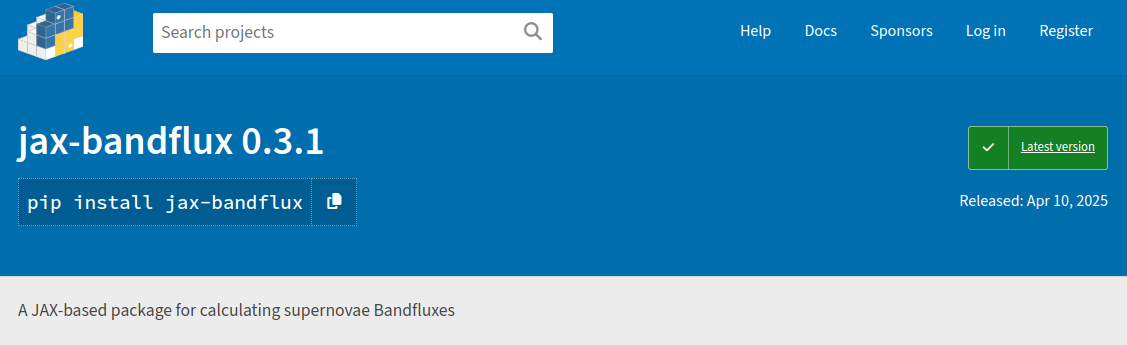
\includegraphics[width=0.55\columnwidth]{talk/images/pip-jax-bandflux.png} &
    
\includegraphics[width=0.25\columnwidth]{talk/images/jax_logo_250px.png}
    \end{tabular}
    
    % Right column - Images
    \column{0.48\textwidth}
    
    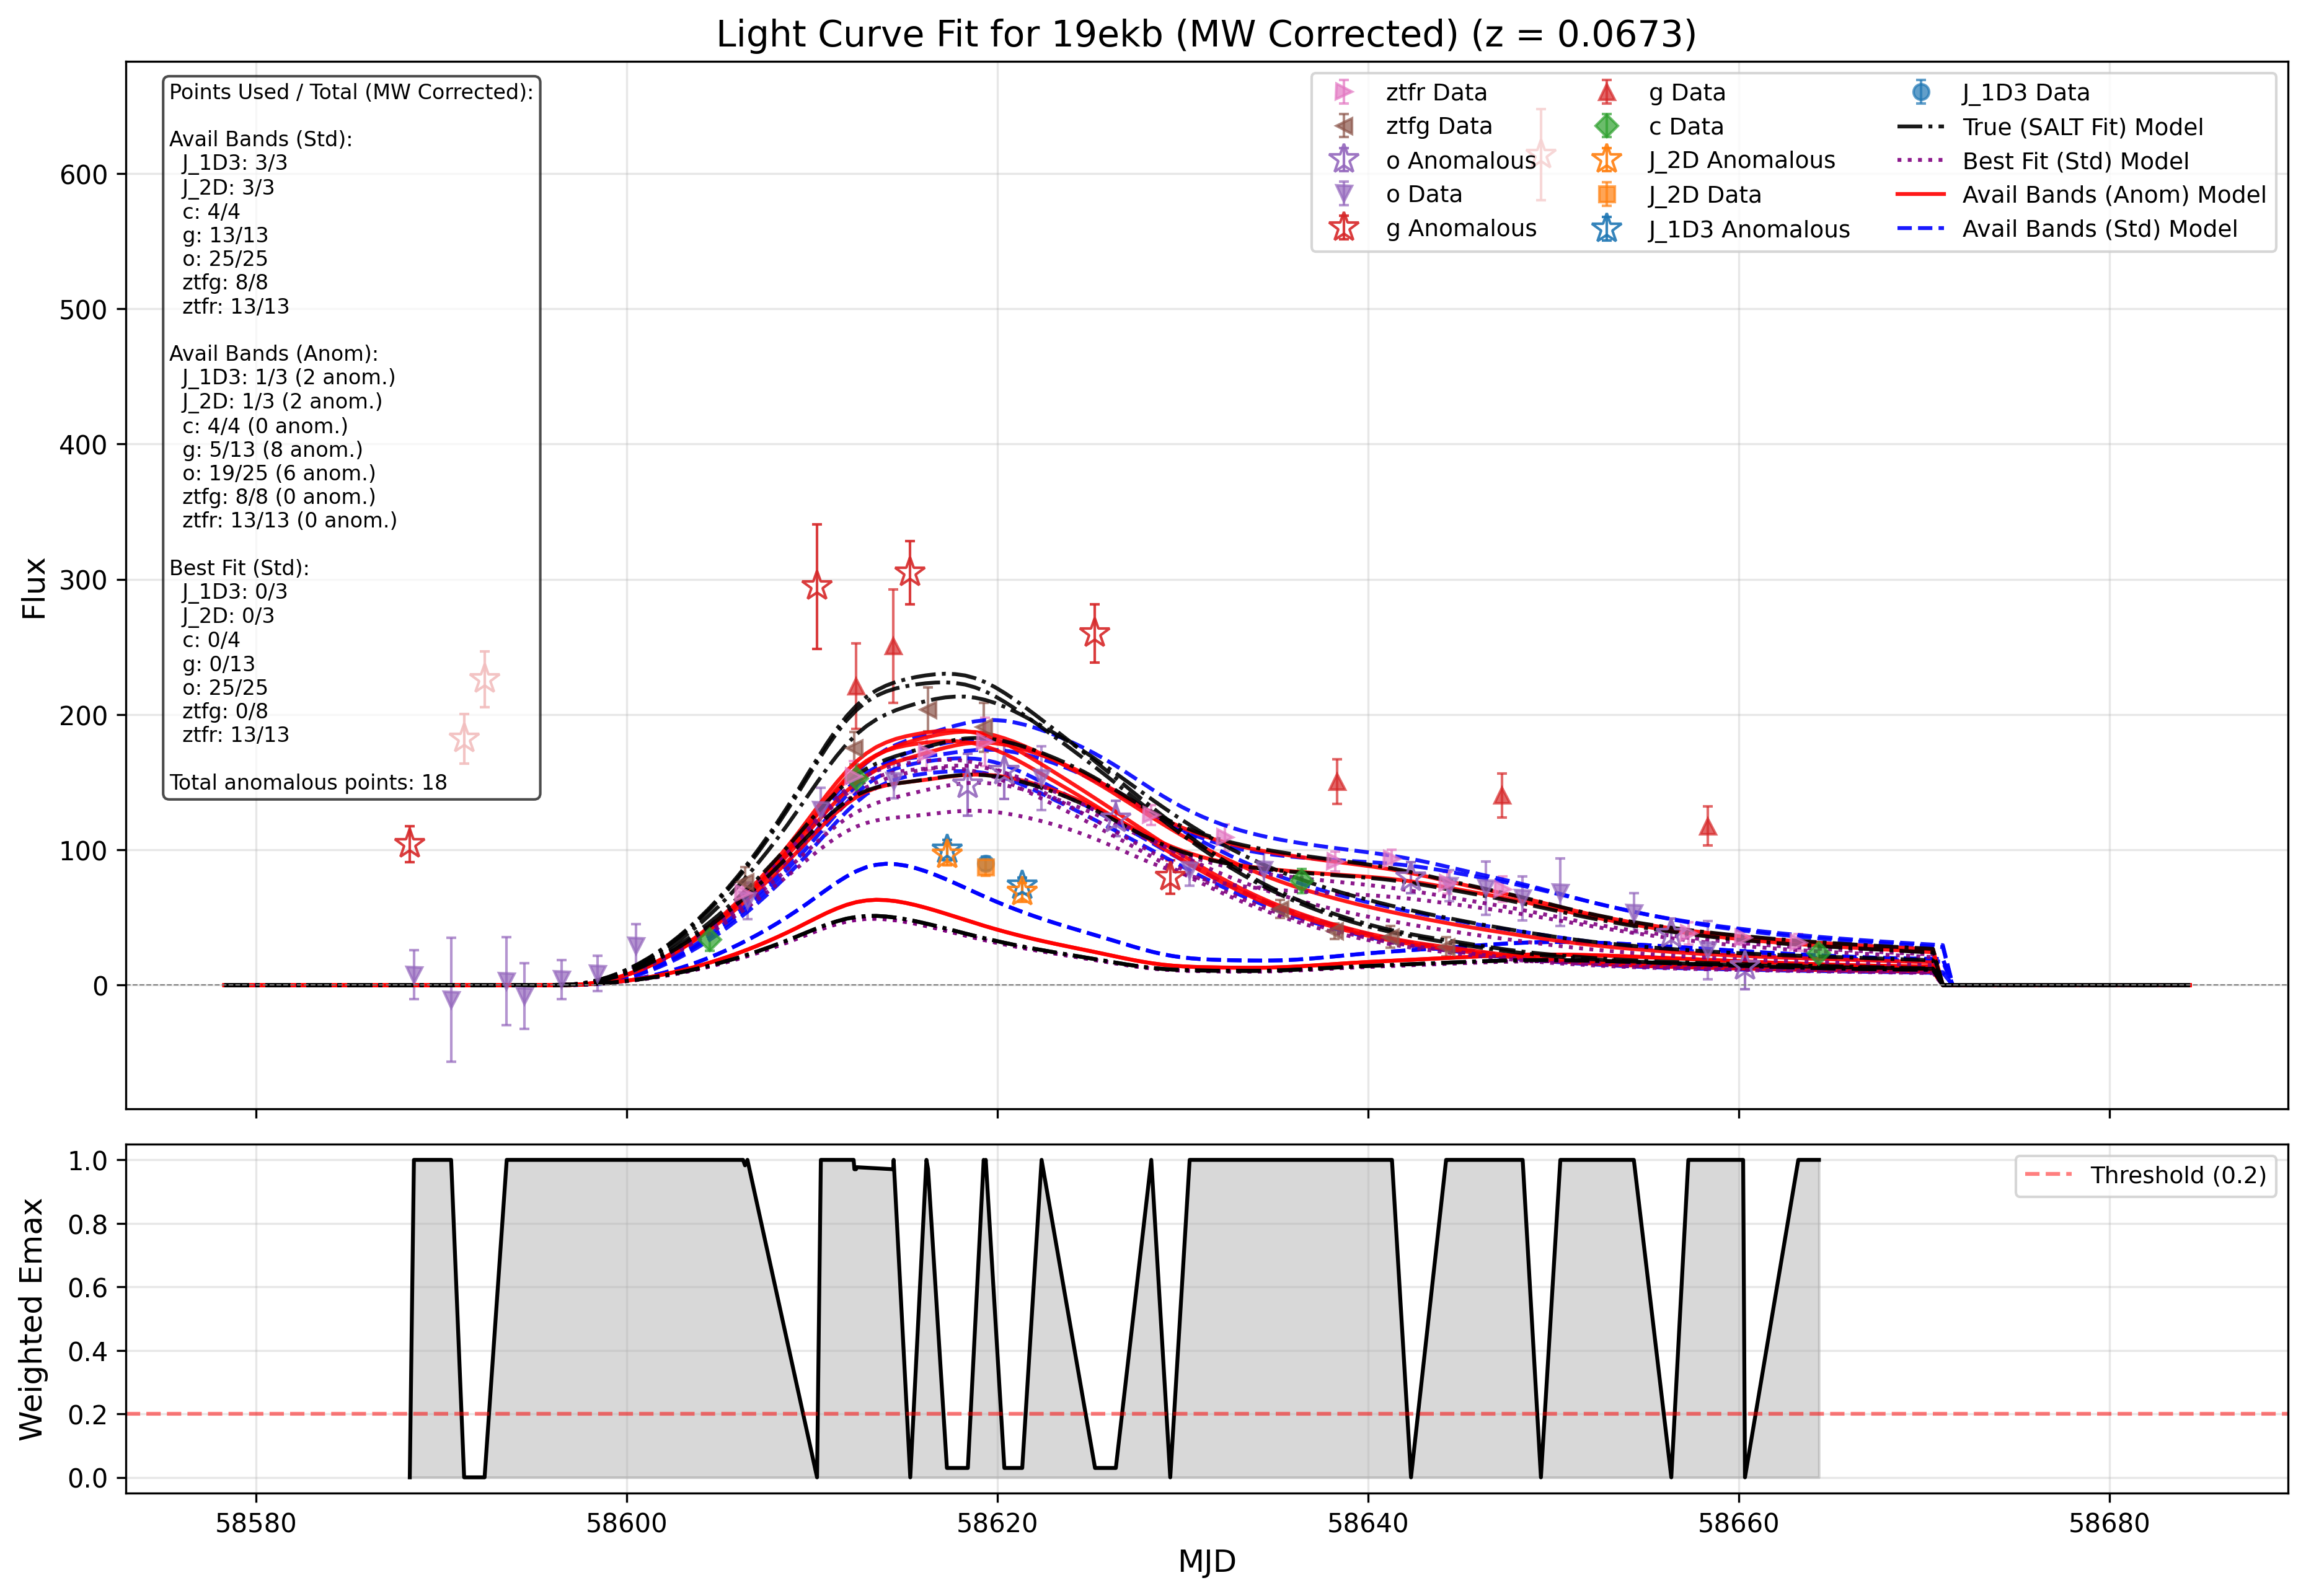
\includegraphics[width=0.7\textwidth]{posters/light_curve_comparison_19ekb_mwcorr.png}
    
    \vspace{0.05cm}
    
    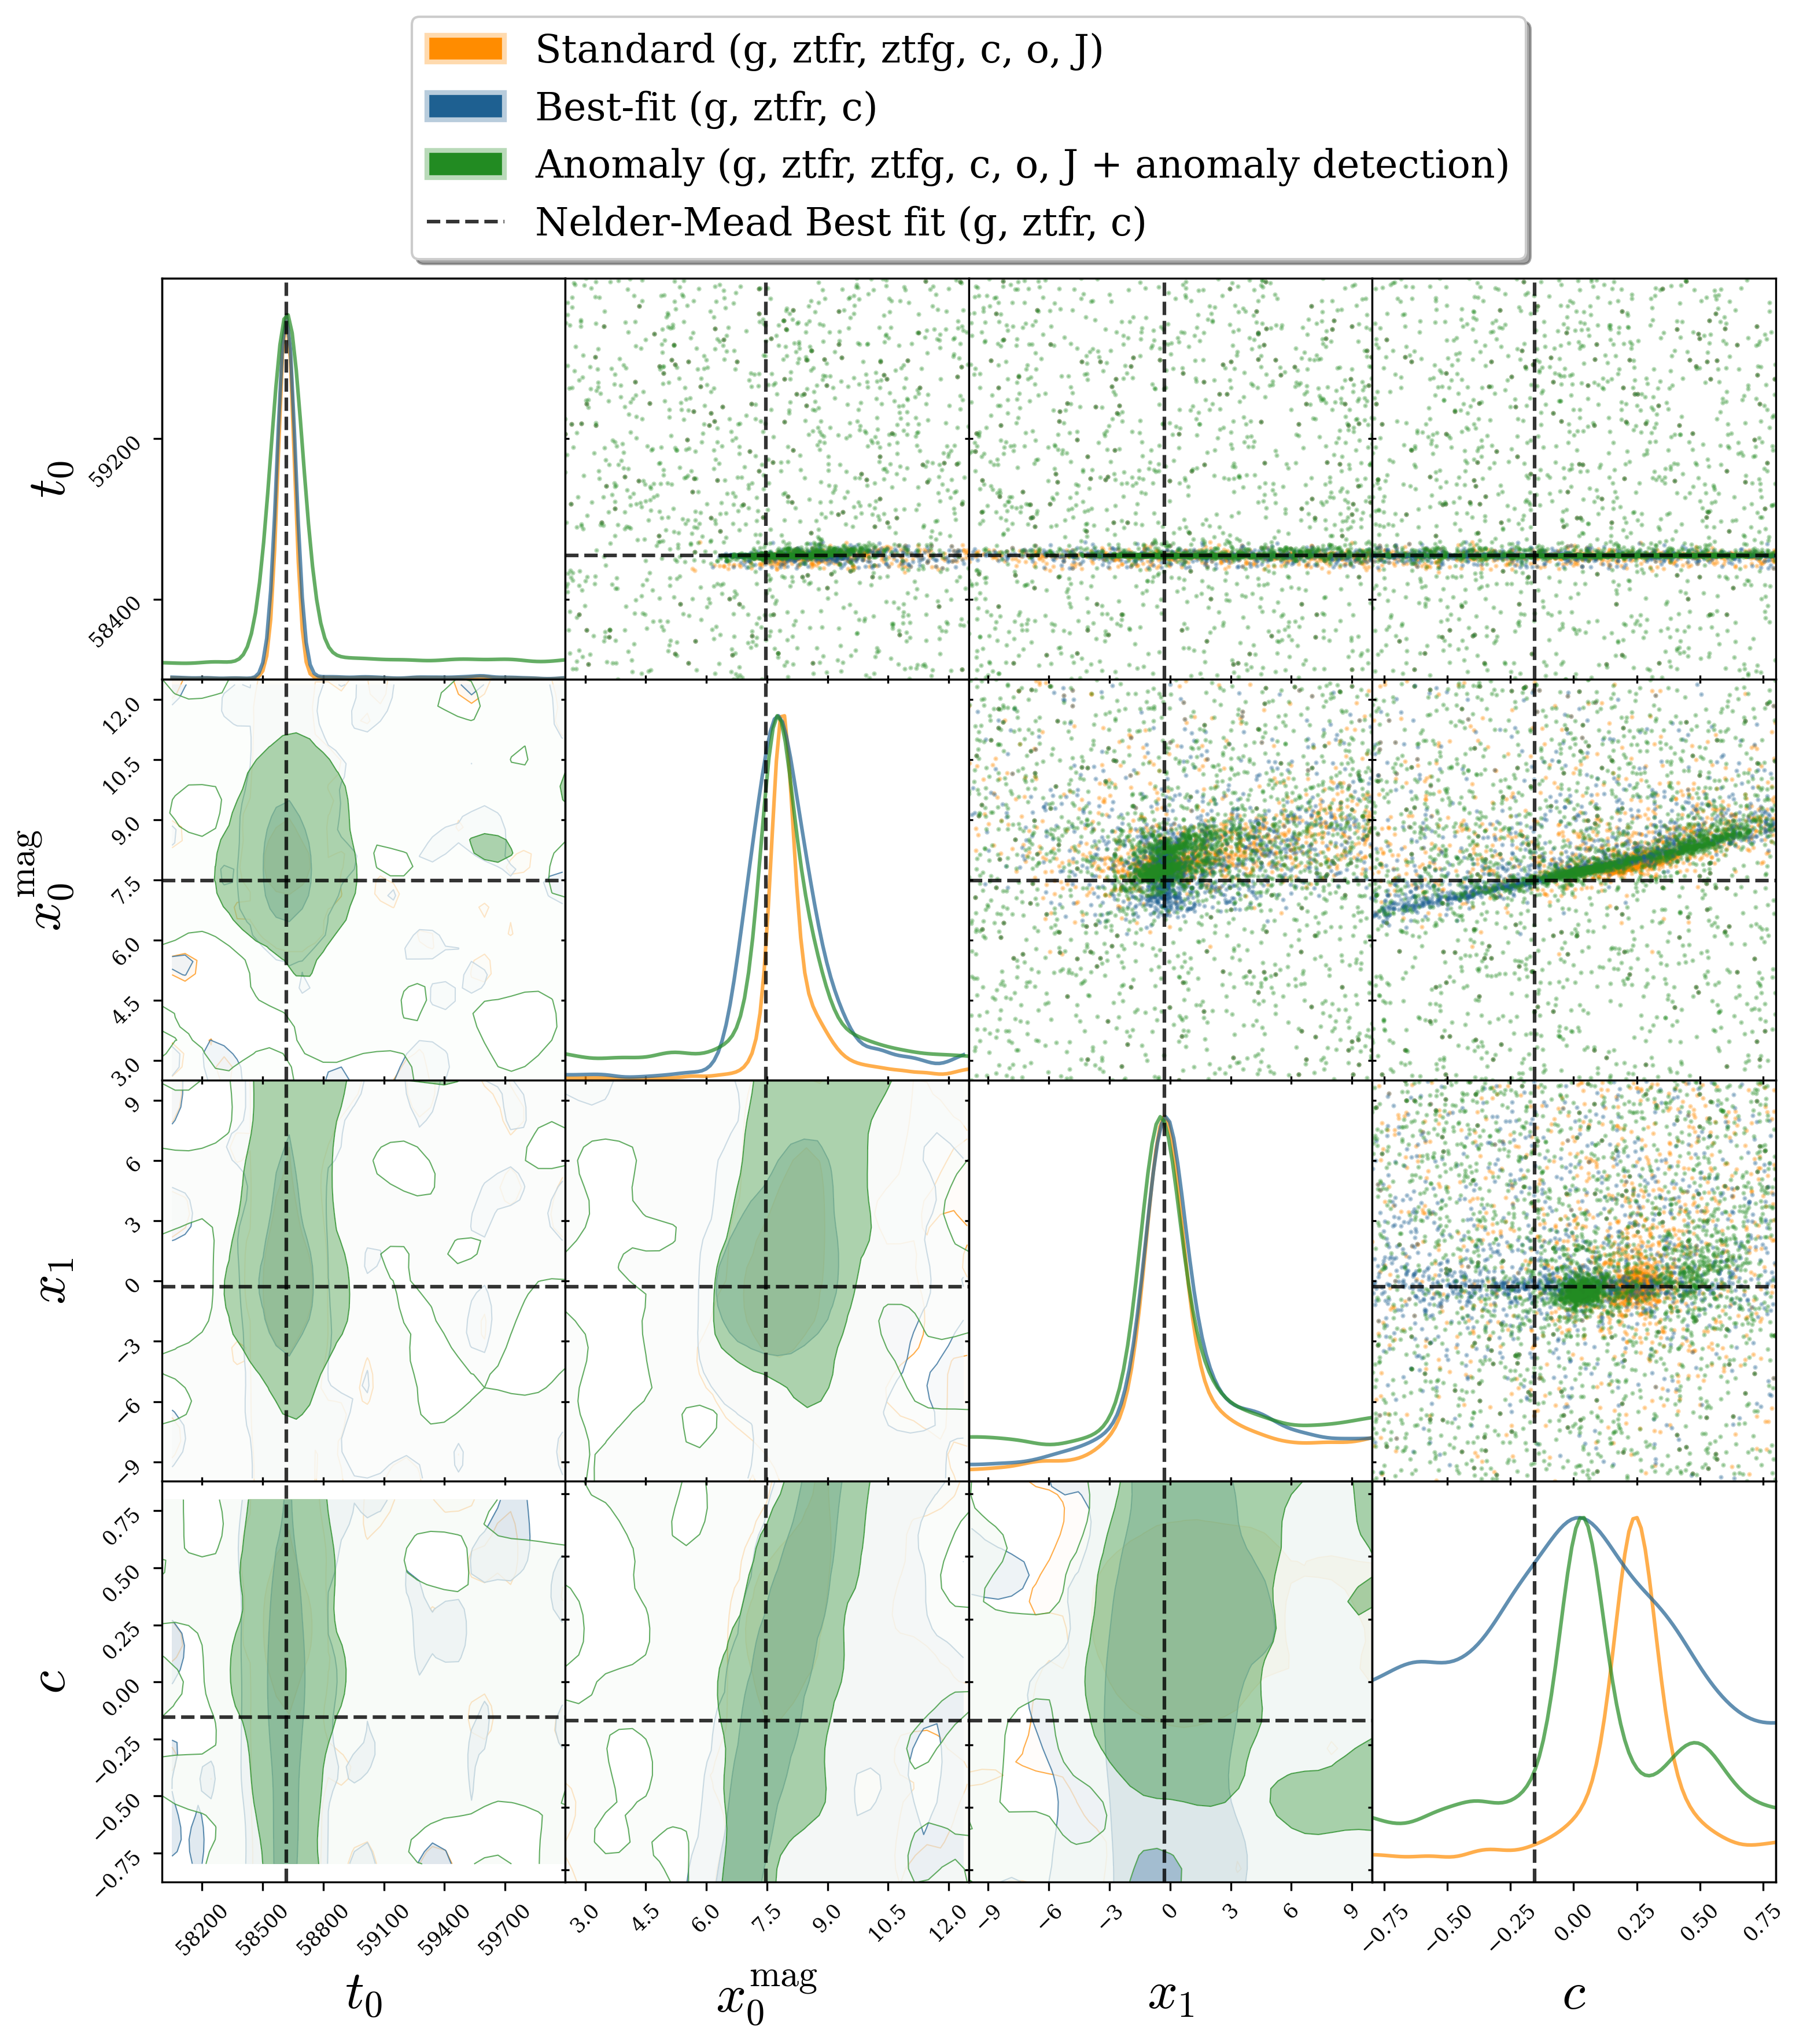
\includegraphics[width=0.7\textwidth]{posters/corner_comparison_19ekb_paper_quality.png}
    
  \end{columns}
\end{frame}

\end{document}